\documentclass[hidelinks,12pt]{article}
\usepackage{graphicx}
\usepackage{amsmath, amssymb}
\usepackage{hyperref}
\usepackage{overpic}
\usepackage{booktabs}
\usepackage{subcaption}
\usepackage{fancyhdr}
\usepackage[dvipsnames]{xcolor}
\usepackage{titlesec}
\usepackage{caption}
\usepackage{lipsum}
\usepackage[a4paper,left=2cm,right=2cm,top=2.5cm,bottom=2.5cm]{geometry}
\usepackage{indentfirst}
\usepackage{placeins}
\usepackage{cleveref}
\usepackage{url}
\renewcommand{\theequation}{\Roman{equation}}

\pagestyle{fancy}
\fancyhf{}
\cfoot{\thepage}
\setlength{\parindent}{0pt}


\begin{document}
	
	\begin{titlepage}
		\begin{center}
			
\includegraphics[width=10cm]{figures/SUT_logo.png} \\
			\vspace{1cm}
			\textbf{\Large Theory of Electrical Circuits PROJECT}\\
			\vspace{0.5cm}
			\textbf{Instructor: Prof. Mostafa Zarghani}\\
			\vspace{1cm}
			\textbf{SHARIF UNIVERSITY OF TECHNOLOGY}\\
			\vspace{1cm}
			\rule{\linewidth}{0.5mm} \\
			\vspace{0.5cm}
			{\Huge \textbf{Twin-T Notch Filter}}\\
			\vspace{0.3cm}
			\rule{\linewidth}{0.5mm} \\
			\vfill
			\textbf{\Large S.K. Pishbin}
			\\
			\textbf{\Large M.M. Roshani}
		\end{center}
	\end{titlepage}
	
	\tableofcontents
	
	\newpage
	\section{Summary}
	Noise reduction in electronic circuits is essential for signal integrity, particularly to mitigate 50~Hz or 60~Hz power line interference using notch filters. This report details the design, simulation, and analysis of a notch filter, initially targeting 60~Hz interference and subsequently adapted for 50~Hz. It also explores the impact of component tolerances through Monte Carlo simulations and includes an experimental setup to validate the theoretical results. This project was partially based on the Texas Instruments application note "High-speed Notch Filters" \cite{TI_slyt235}.
	
	
	\section{Methodology}
	\subsection{Notch Filter Design}
	A Twin-T notch filter was designed to eliminate 50~Hz noise. The circuit components were selected to achieve the desired notch depth and quality factor ($Q$). The governing equation for the center frequency is:
	\begin{equation} \label{eq:1}
		f_0 = \frac{1}{2\pi R_0 C_0}
	\end{equation}
	where $R_0$ and $C_0$ are the primary resistance and capacitance values.
	
	\subsection{Monte Carlo Analysis}
	Monte Carlo simulations were used to assess the impact of component tolerances on the filter's performance. Random variations were introduced into the resistor and capacitor values following a normal distribution. The frequency response was analyzed over multiple iterations to evaluate the statistical impact of these tolerances on key performance metrics such as notch depth and bandwidth.
		
	\subsection{Robust Circuit Approach} \label{robust}
	The robust circuit design method increases the circuit's tolerance to variations in component values, ensuring stable and reliable performance. One common technique involves replacing a single resistor with two resistors of half the original value connected in series. This approach reduces the overall deviation in resistance, as individual variations statistically average out, which improves robustness against manufacturing tolerances. Similar techniques can be applied to capacitors and inductors, increasing the circuit's reliability in the presence of component tolerances, temperature variations, and aging effects.
	
	
	\begin{figure}[!h]
		\centering
		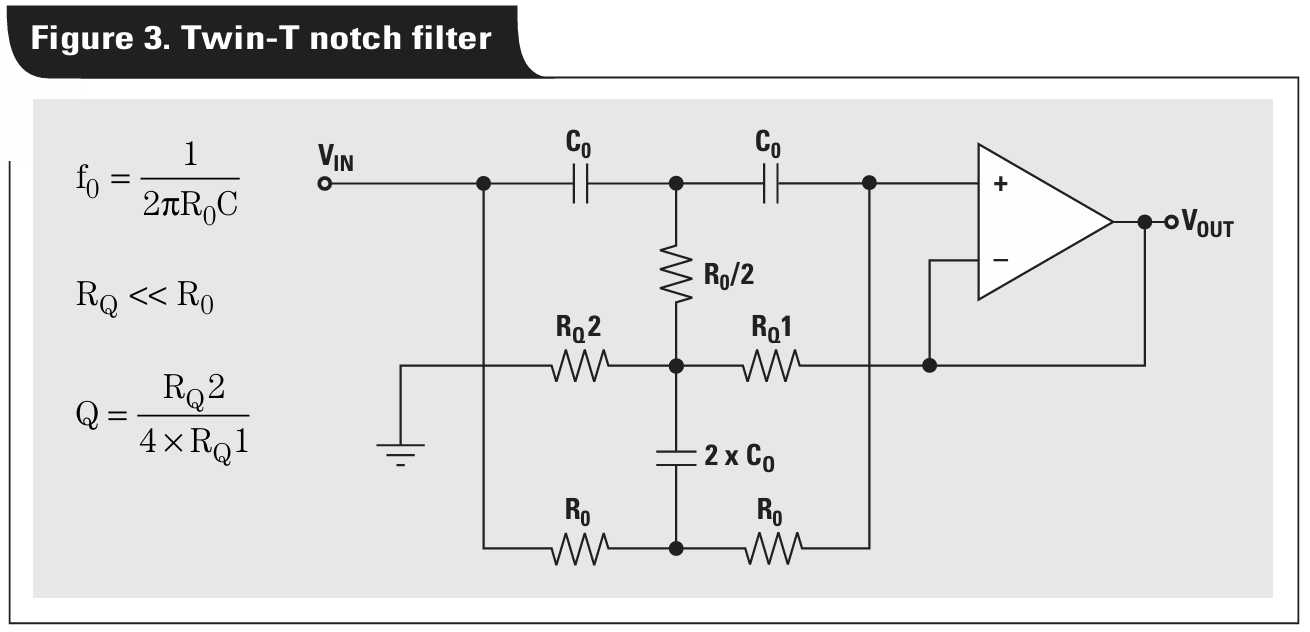
\includegraphics[scale=0.3]{figures/Twin_T.png}
		\caption{Twin-T Notch Filter with \( R_0 \) and \( C_0 \) as Parameters}
	\end{figure}

	\pagebreak
	
	\section{Notch Filter Design and Simulation}
	\subsection{Circuit Analysis}
    \subsubsection{Notch Filter Design for 50~Hz Noise Elimination}
	In this section, the 60~Hz notch filter is converted to a 50~Hz filter by selecting appropriate values for the capacitors and resistors that influence the filter's center frequency and notch depth. Using \cref{eq:1}, a resistor value of 400 k$\Omega$ is chosen, which results in a corresponding capacitor value of 8 nanofarads.
	
	It should be noted that these values may not be easy to find in practice, so adjustments might be needed. Components can also be combined in series or parallel to get closer to the desired values.
	
	\begin{figure}[!h]
		\centering
			\begin{tabular}{c}
				\begin{subfigure}[t]{0.4\textwidth}
					\centering
					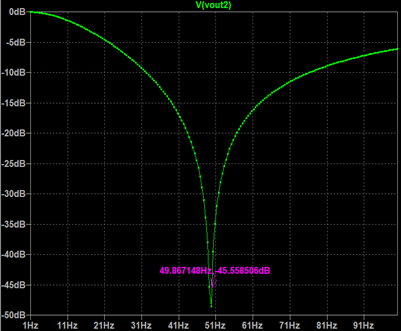
\includegraphics[width=\textwidth]{figures/Notch Filter Design/50hz_freq_response}
					\caption{Frequency Response}
				\end{subfigure}
				\hfill
				\begin{subfigure}[t]{0.45\textwidth}
					\centering
					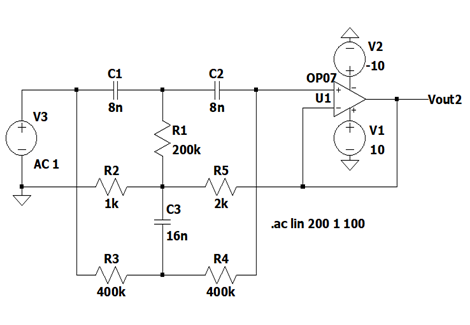
\includegraphics[width=\textwidth]{figures/Notch Filter Design/50hz_circ_design}
					\caption{Circuit Design}
				\end{subfigure} \\
			\end{tabular}
		\caption{50~Hz Notch Filter}
	\end{figure}


    \subsubsection{Q and Its Effect on the Filter}

	Using simulation and the formula \( Q = \frac{R_5}{4R_2} \), we analyze how changes in resistance affect the circuit's frequency response. First, we simulate the initial circuit, where \( Q \) cannot be adjusted, and present its frequency response.
	

	\begin{figure}[!h]
		\centering
			\begin{tabular}{c}
				\begin{subfigure}[t]{0.4\textwidth}
					\centering
					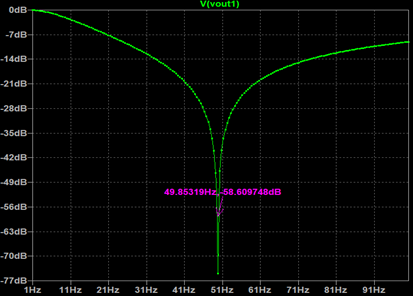
\includegraphics[width=\textwidth]{figures/Notch Filter Design/freq_response_fixed_q}
					\caption{Frequency Response}
				\end{subfigure}
				\hfill
				\begin{subfigure}[t]{0.45\textwidth}
					\centering
					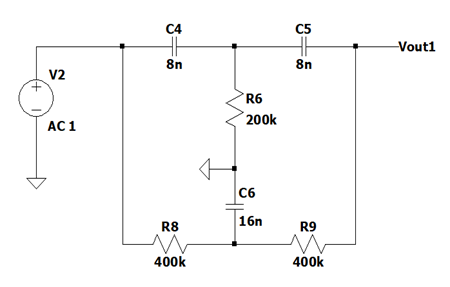
\includegraphics[width=\textwidth]{figures/Notch Filter Design/fixed_q_circuit_design}
					\caption{Circuit Design}
				\end{subfigure} \\
			\end{tabular}
		\caption{Fixed Q Notch Filter}
	\end{figure}


	Next, we present the frequency response and the corresponding circuit with a modified \( Q \) on the notch filter.
	

	\begin{figure}[!h]
		\centering
			\begin{tabular}{c}
				\begin{subfigure}[t]{0.45\textwidth}
					\centering
					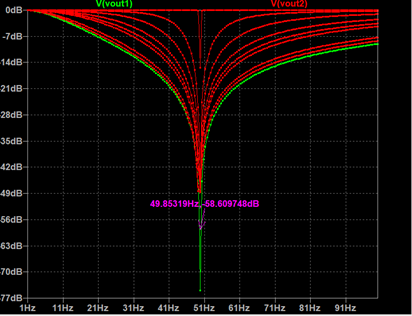
\includegraphics[width=\textwidth]{figures/Notch Filter Design/freq_response_adjustable_q}
					\caption{Frequency Response}
				\end{subfigure}
				\hfill
				\begin{subfigure}[t]{0.5\textwidth}
					\centering
					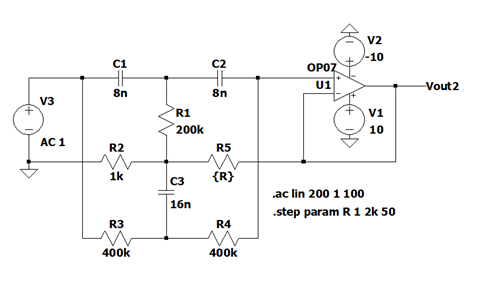
\includegraphics[width=\textwidth]{figures/Notch Filter Design/adjustable_q_circuit}
					\caption{Circuit Design}
				\end{subfigure} \\
			\end{tabular}
		\caption{Adjustable Q}
	\end{figure}

	It can be observed that increasing \( Q \) decreases the filter's bandwidth. By adjusting the resistors \( R_5 \) and \( R_2 \), the desired bandwidth can be achieved.
	\\ \\
	Now, we examine the frequency response at Q \( = 1 \) and calculate the -3~dB bandwidth.

	\begin{figure}[!h]
		\centering
			\begin{tabular}{c}
				\begin{subfigure}[t]{0.45\textwidth}
					\centering
					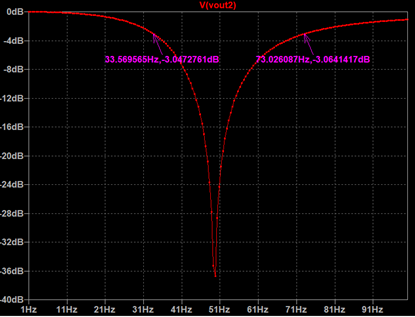
\includegraphics[width=\textwidth]{figures/Notch Filter Design/fre_response_q_1}
					\caption{Frequency Response}
				\end{subfigure}
				\hfill
				\begin{subfigure}[t]{0.5\textwidth}
					\centering
					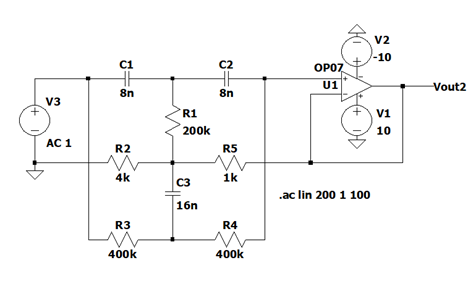
\includegraphics[width=\textwidth]{figures/Notch Filter Design/q_1_circuit_design}
					\caption{Circuit Design}
				\end{subfigure} \\
			\end{tabular}
		\caption{Notch Filter with Q \( = 1 \)}
	\end{figure}

	According to the results, the bandwidth is 40~Hz, ranging from 33~Hz to 73~Hz. Since the noise frequency in Iran varies between 49.8~Hz and 50.2~Hz, increasing \( Q \) too much will significantly reduce the bandwidth, narrowing the oscillation range. This can cause the filter to malfunction and allow noise to pass through.
	
	\pagebreak
	
	\subsubsection{Suitable Operational Amplifier (Op-Amp)}

	For designing a Twin-T Notch Filter aimed at eliminating 50~Hz noise, the op-amp should have the following characteristics:
	

	\begin{enumerate}
		\item \textbf{Suitable Frequency Response:} The op-amp should have a wide enough bandwidth to operate effectively at low frequencies (50~Hz). This ensures the filter will perform well in noise elimination.
		\item \textbf{High Signal-to-Noise Ratio (SNR):} The op-amp should generate minimal noise to maintain signal quality. This feature is crucial for filters where precision is important.
		\item \textbf{Stability at High Frequencies and High Resistor Values:} The op-amp must remain stable in circuits with high resistances (several hundred k$\Omega$) without causing oscillations or distortion.
		\item \textbf{Ability to Operate Accurately with High Resistor Values:} In this project, high-value resistors (several hundred k$\Omega$) will be used, so the op-amp should be well-suited for working with these resistances.
		\item \textbf{High Gain and Linearity:} For precise filter design, the op-amp must provide suitable gain and maintain linearity at low frequencies.
	\end{enumerate}

	\textbf{Two Suggested Models:}

	\begin{itemize}
		\item \textbf{NE5532} \\
		It has a high signal-to-noise ratio and a wide frequency response, offering much more precise performance in 50~Hz noise filters. It also exhibits high stability when using high resistances, making it particularly suitable for designing sensitive and precise filters.
		
		\item \textbf{TL072} \\
		It has a good frequency response and an acceptable signal-to-noise ratio, which is sufficient for most projects. It is suitable for general circuits and analog filters with medium precision, and compared to the NE5532, it is more cost-effective.
	\end{itemize}

	\textbf{Final Conclusion:} If high precision and stability in sensitive circuits are a priority, the \textbf{NE5532} is the best choice. However, if cost and adequate performance within the medium precision range are more important, the \textbf{TL072} would be a suitable option.
	
	\pagebreak
	
	\subsection{Circuit Redesign}

	\subsubsection{Meeting the Desired Conditions}
	Based on the findings from the previous section, we have calculated the circuit components according to the following conditions:

	\[
	\text{BW}_{-3 \, \text{dB}} < 10 \, (\text{Hz}), \quad f_0 = 50 \, (\text{Hz}), \quad \text{Gain}(f = f_0) < -40 \, (\text{dB})
	\]

	\begin{figure}[!h]
		\centering
			\begin{tabular}{c}
				\begin{subfigure}[t]{0.45\textwidth}
					\centering
					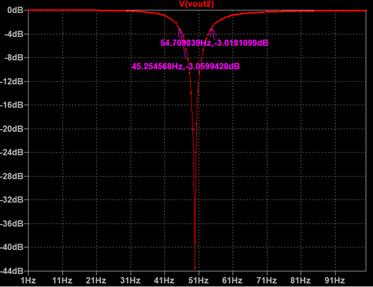
\includegraphics[width=\textwidth]{figures/Notch Filter Design/freq_response_desired}
				\end{subfigure}
				\hfill
				\begin{subfigure}[t]{0.5\textwidth}
					\centering
					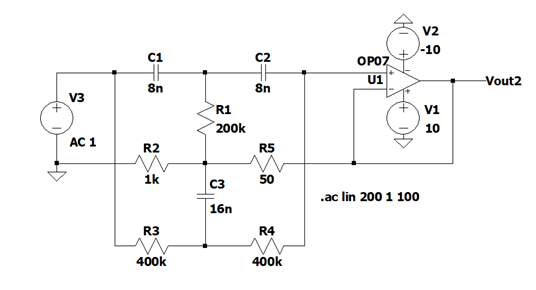
\includegraphics[width=\textwidth]{figures/Notch Filter Design/desired_circuit}
				\end{subfigure}
			\end{tabular}
		\caption{Frequency Response and Circuit Design for Notch Filter with Desired Conditions}
	\end{figure}

	\subsubsection{Design Based on the Standard and Available Values}
	Now, we modify the main components of the circuit that form the notch filter at 50~Hz based on standard market-available values to achieve the desired result with the fewest number of resistors and capacitors. The circuit can be selected from the three options below. It should be noted that the values of the capacitors and resistors are based on the E24 series, and their values can be adjusted by multiplying or dividing them by factors of 10.

	\begin{figure}[!h]
		\centering
			\begin{tabular}{c}
				\begin{subfigure}[t]{0.33\textwidth}
					\centering
					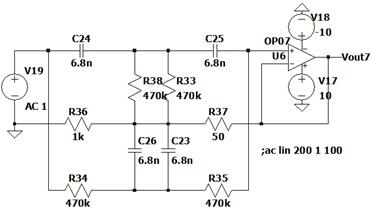
\includegraphics[width=\textwidth]{figures/Notch Filter Design/design_1}
					\caption{}
				\end{subfigure}
				\hfill
				\begin{subfigure}[t]{0.33\textwidth}
					\centering
					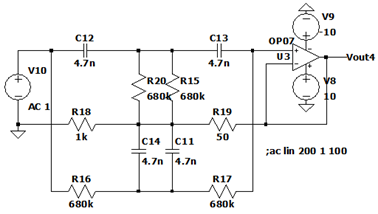
\includegraphics[width=\textwidth]{figures/Notch Filter Design/design_2}
					\caption{}
					\label{fig:chosen_circuit}
				\end{subfigure}
				\hfill
				\begin{subfigure}[t]{0.33\textwidth}
					\centering
					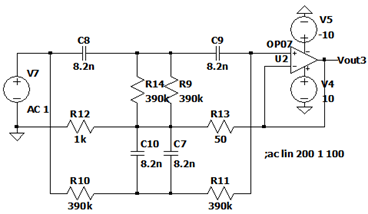
\includegraphics[width=\textwidth]{figures/Notch Filter Design/design_3}
					\caption{}
				\end{subfigure}
			\end{tabular}
		\caption{Circuit Designs for Notch Filter with Standard Components}
	\end{figure}


	\pagebreak
	
	\section{Transfer Function}
	From the circuits designed in the previous section, we have selected \cref{fig:chosen_circuit}. In the subsequent sections, the naming conventions will be based on the following circuit.
	
	\begin{figure}[!h]
		\centering
		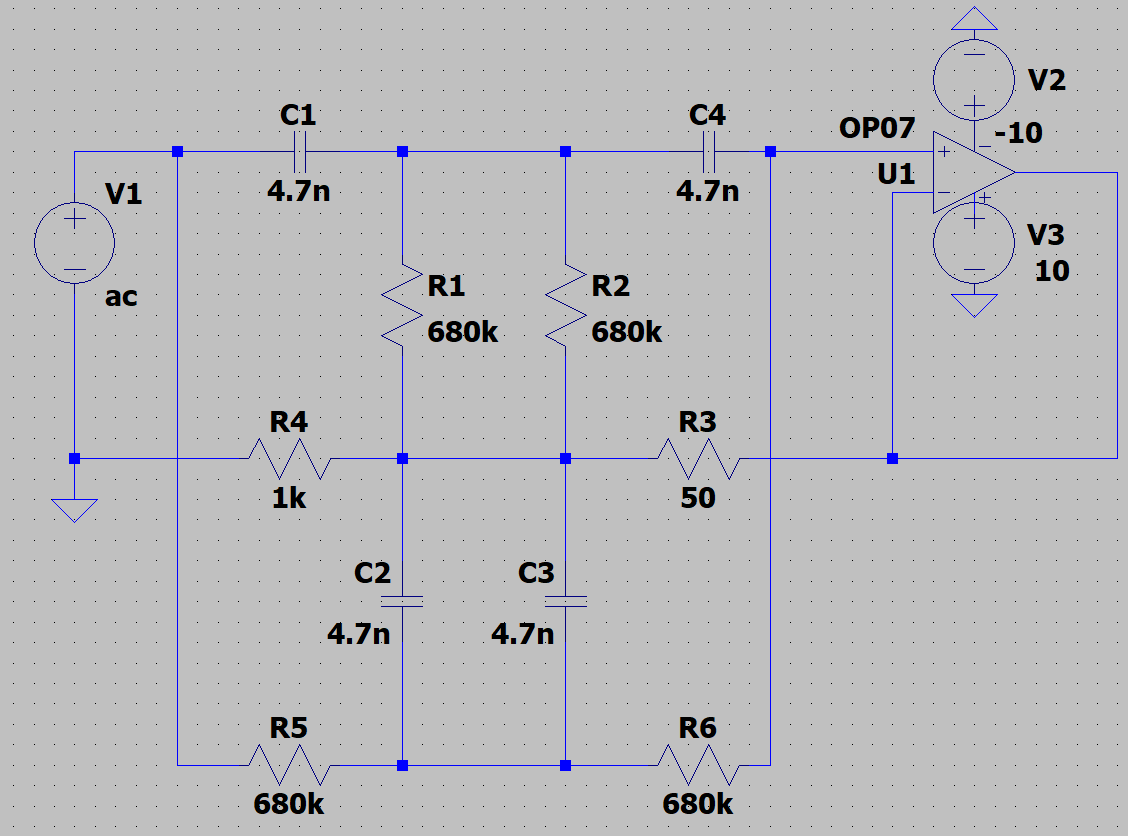
\includegraphics[scale=0.4]{figures/base_circuit_phase_2.png}
		\caption{The Selected Circuit for Implementation}
	\end{figure}
	
	
	\subsection{Transfer Function Calculation}
	To calculate the transfer function, we used the admittance matrix approach in MATLAB. Instead of directly solving the system of equations, we represented the circuit using its admittance matrix, which is a more efficient method for handling complex systems. This method allows us to perform matrix multiplication and inversion to derive the transfer function. \\
	The component values were set as \( R_{3} = 50\,\Omega \) and \( R_{4} = 1\,\text{k}\Omega \). Kirchhoff's Current Law (KCL) equations were formulated for the circuit and converted into admittance matrix form. The resulting admittance matrix is:
	

	$$
	\begin{bmatrix}
		-Y_{C4} & Y_{C1} + Y_1 + Y_2 + Y_{C4} & -Y_1 - Y_2 & 0 \\
		Y_{C4} + Y_6 & -Y_{C4} & 0 & -Y_6 \\
		-Y_3 & -Y_1 - Y_2 & (Y_{C2} + Y_{C3}) + Y_1 + Y_2 + Y_3 + Y_4 & -(Y_{C2} + Y_{C3}) \\
		-Y_6 & 0 & -(Y_{C2} + Y_{C3}) & Y_5 + Y_6 + (Y_{C2} + Y_{C3})
	\end{bmatrix}
	$$
	\newline
	Finally, the transfer function \( H(s) \) of the circuit, derived from the admittance matrix, is given by:

	$$
	H(s) = 
	\frac{21\,{C_0 }^2 \,{R_0 }^2 \,s^2 + 4000\,{C_0 }^2 \,R_0 \,s^2 + 4000\,C_0 \,s + 21}{21\,{C_0 }^2 \,{R_0 }^2 \,s^2 + 4000\,{C_0 }^2 \,R_0 \,s^2 + 4\,C_0 \,R_0 \,s + 4000\,C_0 \,s + 21}
	$$
	\newline
	Using the admittance matrix method simplifies the process of obtaining the transfer function, making it easier to manipulate and analyze the system’s behavior.
			
	\pagebreak
	
	\subsection{Bode Diagram}
		Now that we have obtained the transfer function, we can substitute the values calculated in the previous section. We set $R_0 = 680\,\text{k}\Omega$, $C_0 = 4.7\,\text{nF}$, and $s = j\omega$, where \( j \) represents the imaginary unit and \( \omega \) is the angular frequency. With these values, we can plot the Bode diagram.

		\begin{figure}[!h]
			\centering
			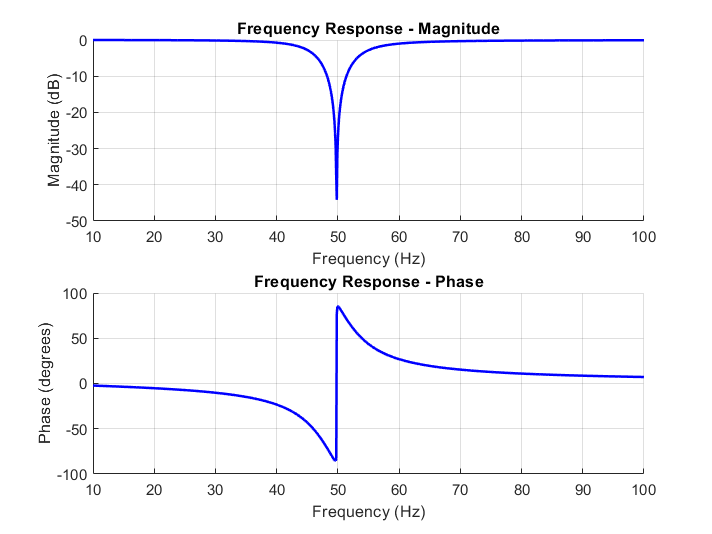
\includegraphics[scale=0.8]{figures/bode_diagram.png}
			\caption{Bode Diagram of the Transfer Function}
		\end{figure}

	The magnitude plot of the frequency response reveals that the circuit attenuates the signal around 50~Hz, which aligns with the desired behavior for this filter.
	

	
	\pagebreak
	
	\section{Monte Carlo Analysis}
	In our Monte Carlo analysis, we assume that the values of the circuit elements are random variables following a Gaussian distribution. The mean of each distribution is the ideal value of the respective component. The effect of different variances (tolerances) will be analyzed in the following sections.
	
	
	\subsection{Monte Carlo Simulation of \( H(j\omega) \) with 2\% Tolerance}
	By setting the tolerance for each element to 2\% and running the simulation 10,000 times, we plot the mean, as well as the first and third quantiles of the aggregate transfer functions. \( R_3 \) and \( R_4 \) are considered ideal.
	
	\begin{figure}[!h]
		\centering
		\begin{subfigure}[t]{0.48\textwidth}
			\centering
			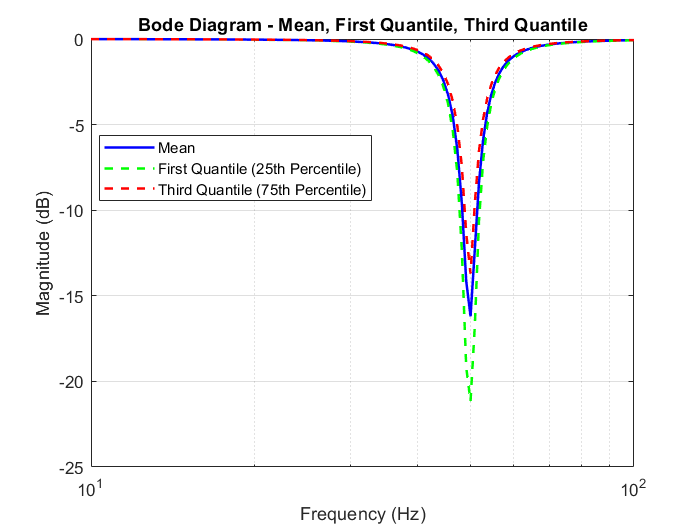
\includegraphics[width=\textwidth]{figures/transfer_function_2_percent_tolerance_all.png}
			\caption{Aggregate Transfer Function}
		\end{subfigure}
		\hfill
		\begin{subfigure}[t]{0.48\textwidth}
			\centering
			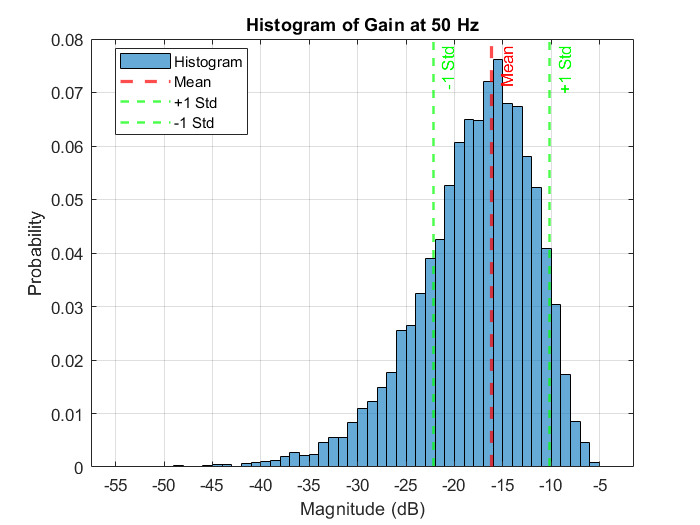
\includegraphics[width=\textwidth]{figures/histogram_gain_50hz_2_percent_tolerance_all.png}
			\caption{Gain Histogram Around 50\,\text{Hz}}
			\label{fig:histogram_gain_50hz}
		\end{subfigure}
		\caption{}
		\label{fig:2_percent_tolerance_all}
	\end{figure}
	
	We can see that the circuit effectively attenuates the signal around 50~Hz, as intended, with the mean gain dropping to approximately -16~dB. The spread between the quantile curves reflects the variability introduced by component tolerances.
	
	\pagebreak
	
	
	\subsection{Effect of 5\% Tolerance on Each Element}
	Here, we isolate individual circuit elements and plot the gain histogram by assuming a 5\% tolerance for a single element while keeping all other elements at their ideal values. The simulation was performed with 2,000 samples.
	
	\begin{figure}[!h]
		\centering
			\begin{tabular}{c}
				\begin{subfigure}[t]{0.5\textwidth}
					\centering
					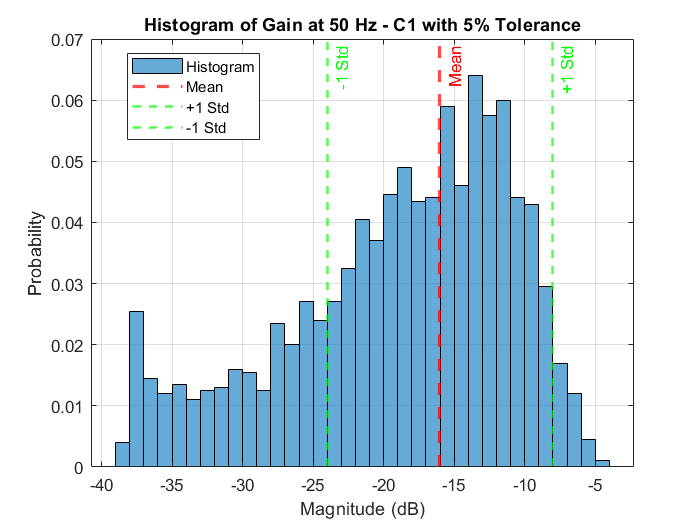
\includegraphics[width=\textwidth]{figures/5_percent/c1.png}
					\caption{$C_1$}
				\end{subfigure}
				\hfill
				\begin{subfigure}[t]{0.5\textwidth}
					\centering
					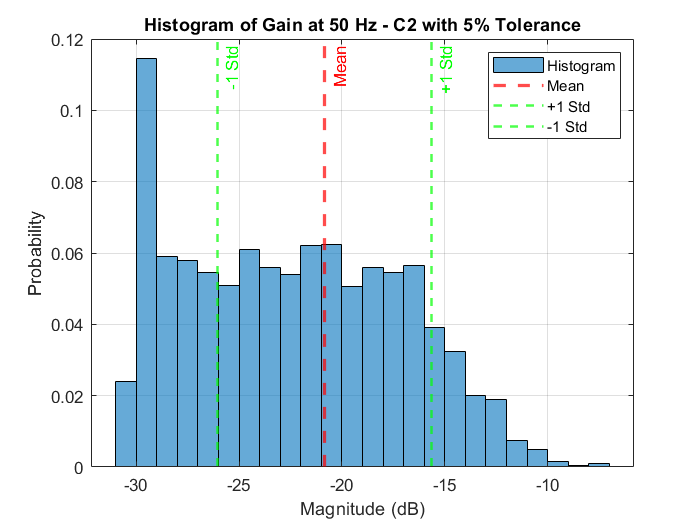
\includegraphics[width=\textwidth]{figures/5_percent/c2.png}
					\caption{$C_2$}
				\end{subfigure} \\
				
				\begin{subfigure}[t]{0.5\textwidth}
					\centering
					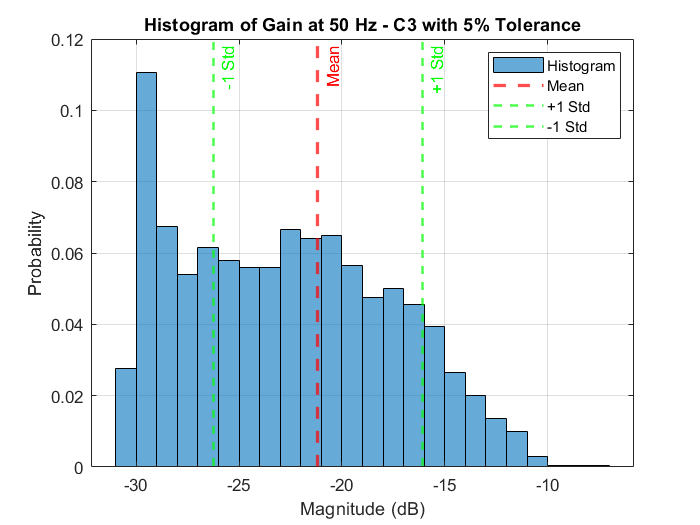
\includegraphics[width=\textwidth]{figures/5_percent/c3.png}
					\caption{$C_3$}
				\end{subfigure}
				\hfill
				\begin{subfigure}[t]{0.5\textwidth}
					\centering
					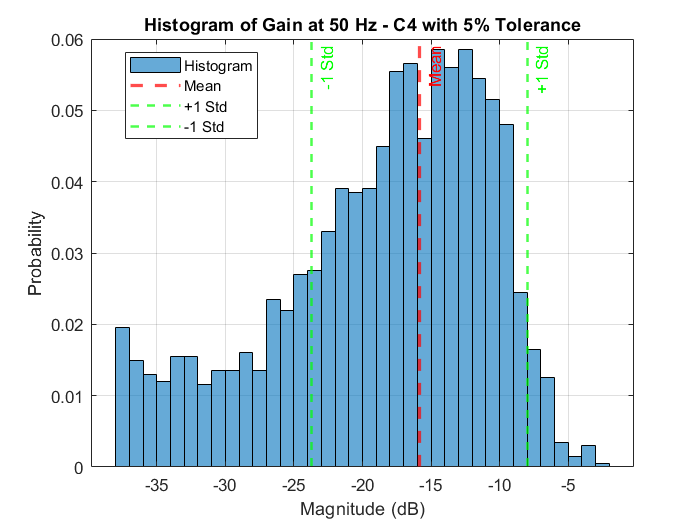
\includegraphics[width=\textwidth]{figures/5_percent/c4.png}
					\caption{$C_4$}
				\end{subfigure}
			\end{tabular}
		\caption{Gain Histograms for Capacitors with 5\% Tolerance}
	\end{figure}
	
	\pagebreak
	
	% Resistors (R1 to R6) - 3x2 Grid Layout
	\begin{figure}[!h]
		\centering
		\begin{tabular}{cc}
			\begin{subfigure}[h]{0.45\textwidth}
				\centering
				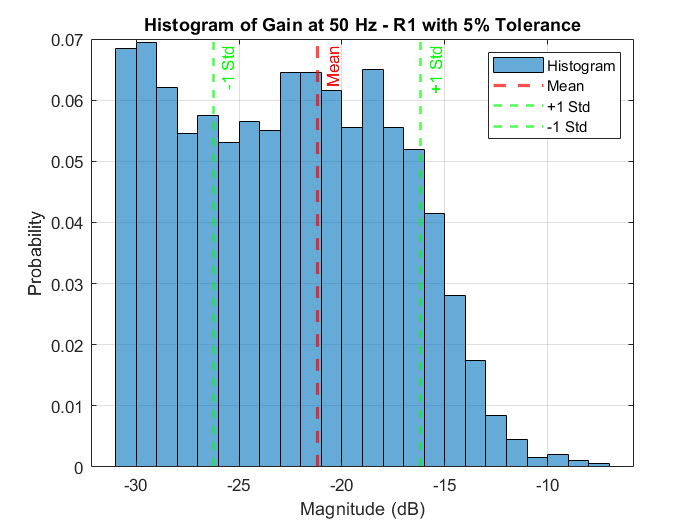
\includegraphics[width=\textwidth]{figures/5_percent/r1.png}
				\caption{$R_1$}
			\end{subfigure} &
			\begin{subfigure}[h]{0.45\textwidth}
				\centering
				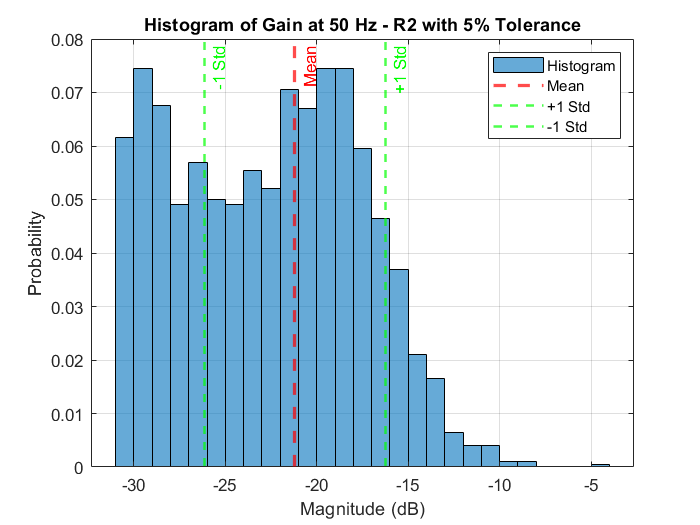
\includegraphics[width=\textwidth]{figures/5_percent/r2.png}
				\caption{$R_2$}
			\end{subfigure} \\[0.3cm]
			
			\begin{subfigure}[h]{0.45\textwidth}
				\centering
				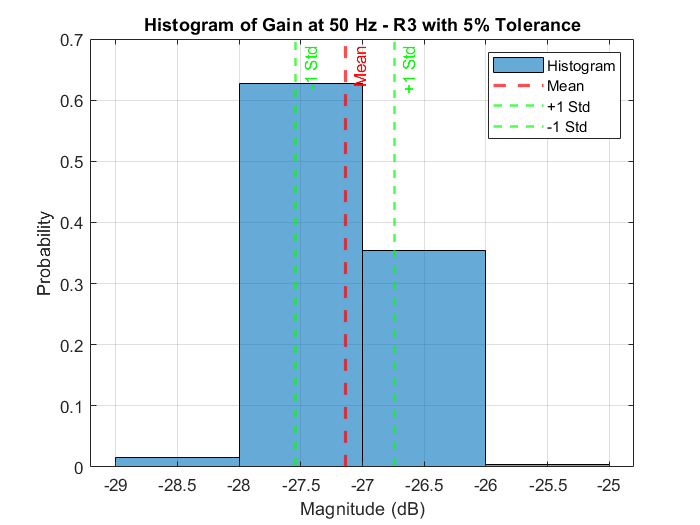
\includegraphics[width=\textwidth]{figures/5_percent/r3.png}
				\caption{$R_3$}
			\end{subfigure} &
			\begin{subfigure}[h]{0.45\textwidth}
				\centering
				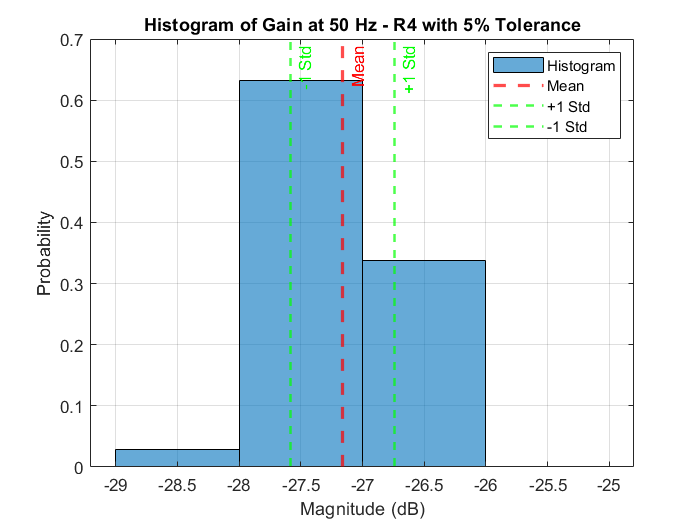
\includegraphics[width=\textwidth]{figures/5_percent/r4.png}
				\caption{$R_4$}
			\end{subfigure} \\[0.3cm]
			
			\begin{subfigure}[h]{0.45\textwidth}
				\centering
				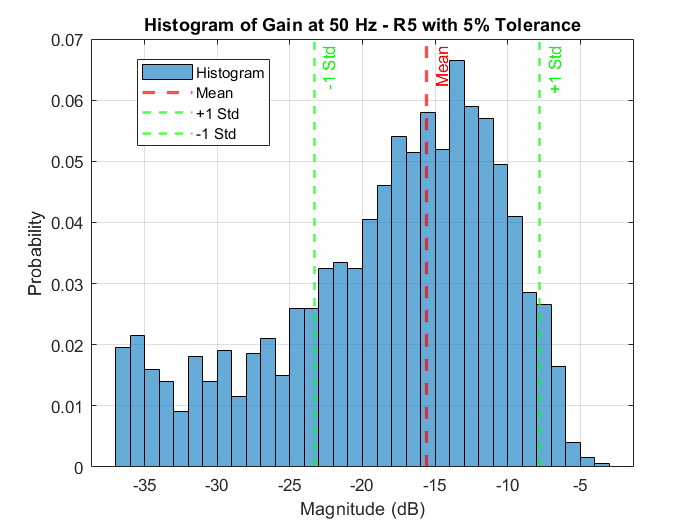
\includegraphics[width=\textwidth]{figures/5_percent/r5.png}
				\caption{$R_5$}
			\end{subfigure} &
			\begin{subfigure}[h]{0.45\textwidth}
				\centering
				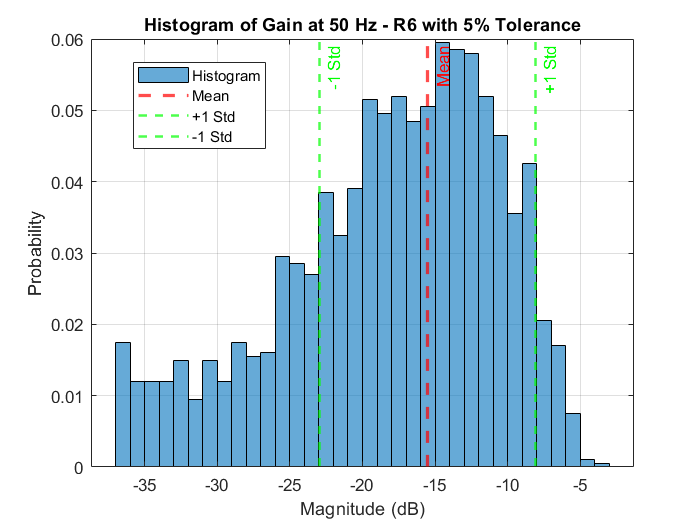
\includegraphics[width=\textwidth]{figures/5_percent/r6.png}
				\caption{$R_6$}
			\end{subfigure}
		\end{tabular}
		\caption{Gain Histograms for Resistors with 5\% Tolerance}
		\label{fig:resistors_5_percent}
	\end{figure}
	

	Based on the results, we observe that the circuit is more sensitive to tolerances in certain elements, specifically \( \{C_1, C_4, R_5, R_6\} \), while variations in other elements do not have as much of an impact on the circuit's performance.
	
	\pagebreak
	
	\subsection{Adjusting Q to Achieve a More Reliable Circuit}
	\textbf{Question: }Now, based on the obtained results, try to determine an optimal tolerance for each element so that the following conditions are met. Guidance: You may need to adjust \( Q \) to satisfy some of the conditions. Use the new values of \( R_3 \) and \( R_4 \) in the continuation of the project.
	
	\begin{equation} \label{eq:constraints}
		BW_{-3\text{dB}} < 25\,\text{Hz}, \quad f_o = 50\,\text{Hz}, \quad P(\text{Gain at 50\,Hz} < -20\,\text{dB}) > 0.9
	\end{equation}
	\\ \\
	Given the results in the previous section, we observe that the target frequency response of \( P(\text{Gain at 50\,Hz} < -20\,\text{dB}) > 0.9 \) is rarely achieved. There are multiple ways to bridge this gap. We can:
	
	\begin{itemize}
		\item Use elements with lower tolerances
		\item Lower the Q
		\item Use a second filter
	\end{itemize}
	The first option, using elements with lower tolerances, is not feasible due to availability or high cost. Since we are designing a single filter, the third option, adding a second filter, is also unsuitable. Therefore, our last resort is to reduce the \( Q \), sacrificing some accuracy for improved tolerance insensitivity. A trade-off exists between accuracy and the -3~dB bandwidth. To achieve the best results within these constraints, we set \( BW_{-3\text{dB}} = 25\,\text{Hz} \) and simulate different \( R_3 \) values. Using E24 resistor values, we test \( R_3 \) values of 130, 150, and 180 to find the closest match to a 25~Hz bandwidth. \\ \\
	
	\begin{figure}[!h]
		\centering
		\begin{overpic}[width=1\textwidth]{figures/r3_130.png}
			\put(63,2){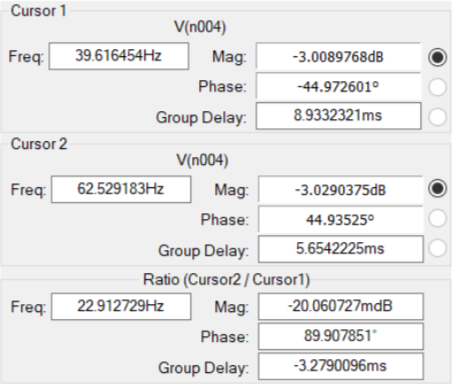
\includegraphics[width=0.35\textwidth]{figures/r3_130_caption.png}}
		\end{overpic}
		\caption{$R_3 = 130$}
	\end{figure}
	
	\begin{figure}[!h]
		\centering
		\begin{overpic}[width=1\textwidth]{figures/r3_150.png}
			\put(63,2){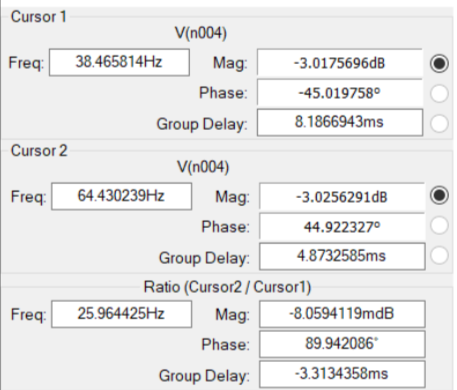
\includegraphics[width=0.35\textwidth]{figures/r3_150_caption.png}}
		\end{overpic}
		\caption{$R_3 = 150$}
	\end{figure}
	
	\begin{figure}[!h]
		\centering
		\begin{overpic}[width=1\textwidth]{figures/r3_180.png}
			\put(63,2){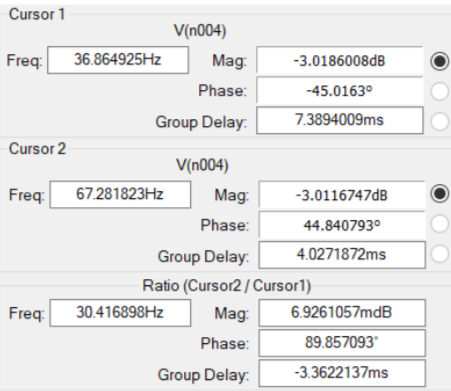
\includegraphics[width=0.35\textwidth]{figures/r3_180_caption.png}}
		\end{overpic}
		\caption{$R_3 = 180$}
	\end{figure}

	\pagebreak

	From the images above, we can summarize the results in the following table:
	
	\begin{table}[h!]
		\centering
		\begin{tabular}{|c|c|}
			\hline
			$R_3$ Value ($\Omega$) & Bandwidth (Hz) \\ \hline
			130                    & 22.9           \\ \hline
			150                    & 25.9           \\ \hline
			180                    & 30.4           \\ \hline
		\end{tabular}
		\caption{\(-3\,\text{dB}\) bandwidth with different values of \(R_3\)}
		\label{tab:R3_bandwidth}
	\end{table}
	
	We see that \( R_3 = 130\,\Omega \) and \( R_3 = 150\,\Omega \) meet our requirements.

	\pagebreak
	
	\subsection{Simulation of \( R_3 \) Values}
	In the previous section, we observed that only \(130\,\Omega\) and \(150\,\Omega\) met our criteria for the \(-3\,\text{dB}\) bandwidth. In this section, we simulate the circuit using these values to determine which one provides a better response. The simulation is performed with 2,000 samples, assuming a 5\% tolerance for a single element while considering all other elements as ideal.
	
	
	\subsubsection{$R_3 = 130\Omega$}

	\begin{figure}[!h]
		\centering
		\resizebox{0.75\textwidth}{!}{
			\begin{tabular}{c}
				\begin{subfigure}[h]{0.4\textwidth}
					\centering
					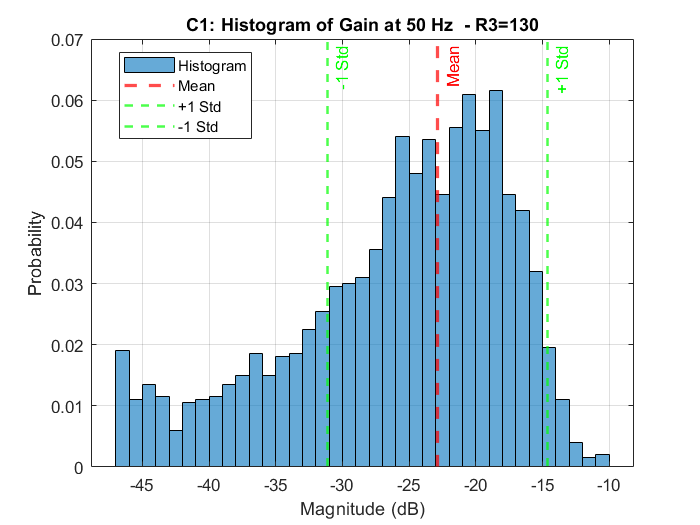
\includegraphics[width=\textwidth]{figures/r3=130/c1.png}
					\caption{$C_1$}
				\end{subfigure}
				\hfill
				\begin{subfigure}[h]{0.4\textwidth}
					\centering
					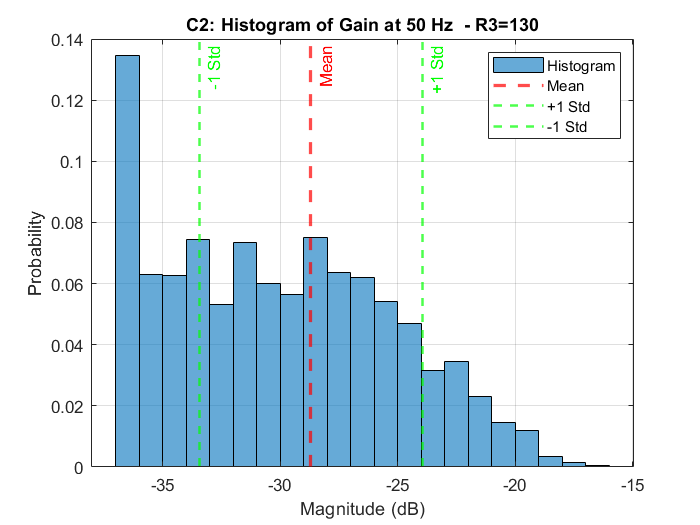
\includegraphics[width=\textwidth]{figures/r3=130/c2.png}
					\caption{$C_2$}
				\end{subfigure} \\
				
				\begin{subfigure}[h]{0.4\textwidth}
					\centering
					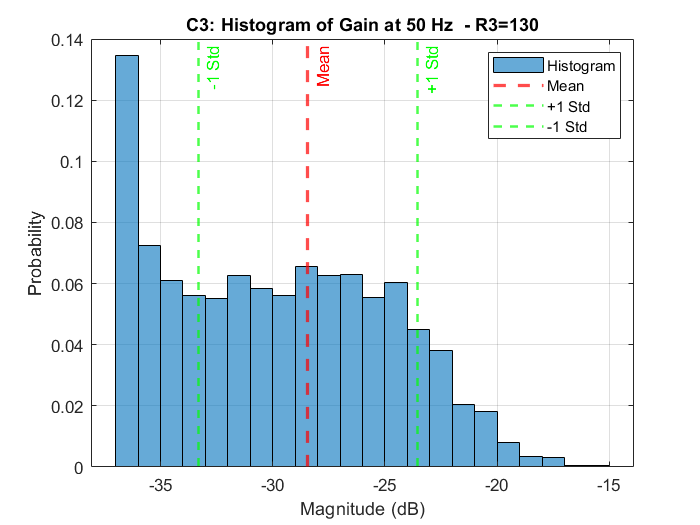
\includegraphics[width=\textwidth]{figures/r3=130/c3.png}
					\caption{$C_3$}
				\end{subfigure}
				\hfill
				\begin{subfigure}[h]{0.4\textwidth}
					\centering
					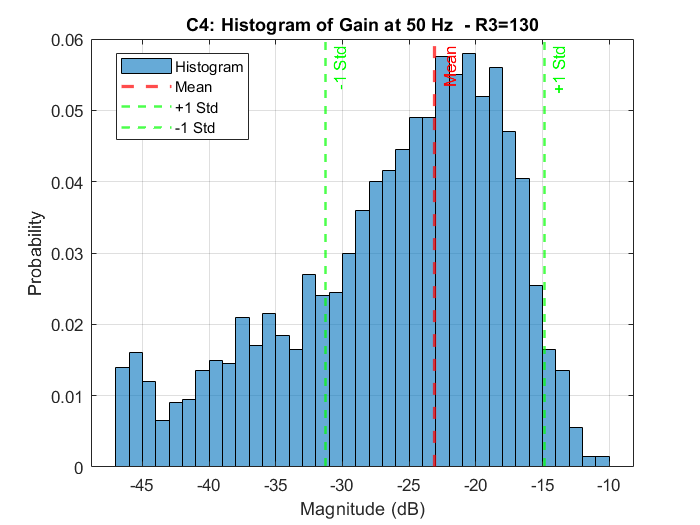
\includegraphics[width=\textwidth]{figures/r3=130/c4.png}
					\caption{$C_4$}
				\end{subfigure}
			\end{tabular}
		}
		\caption{Gain Histograms for Capacitors with 5\% Tolerance}
	\end{figure}
	
	
	
	
	\begin{figure}[!h]
		\centering
		\resizebox{0.75\textwidth}{!}{
			\begin{tabular}{c}
				\begin{subfigure}[h]{0.4\textwidth}
					\centering
					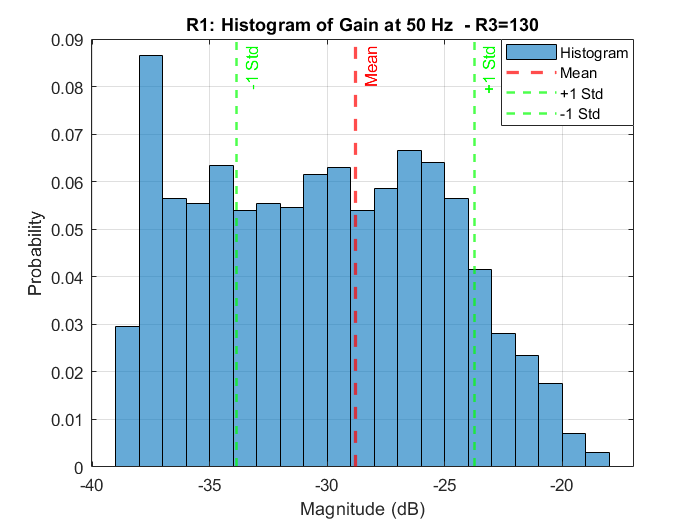
\includegraphics[width=\textwidth]{figures/r3=130/r1.png}
					\caption{$R_1$}
				\end{subfigure}
				\hfill
				\begin{subfigure}[h]{0.4\textwidth}
					\centering
					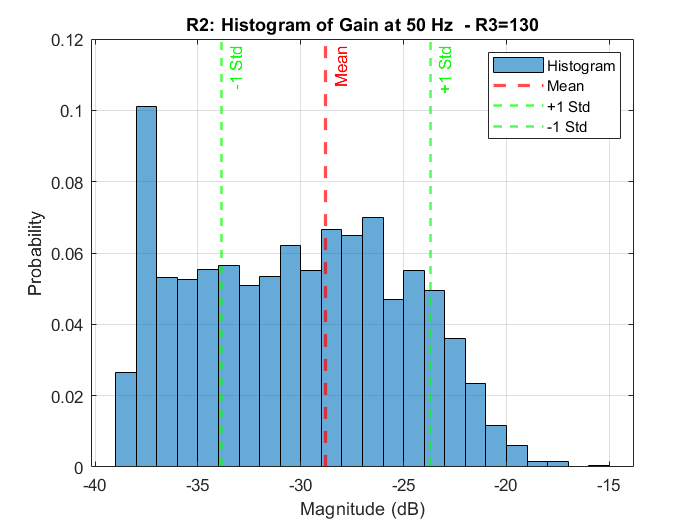
\includegraphics[width=\textwidth]{figures/r3=130/r2.png}
					\caption{$R_2$}
				\end{subfigure}
				\hfill
				\begin{subfigure}[h]{0.4\textwidth}
					\centering
					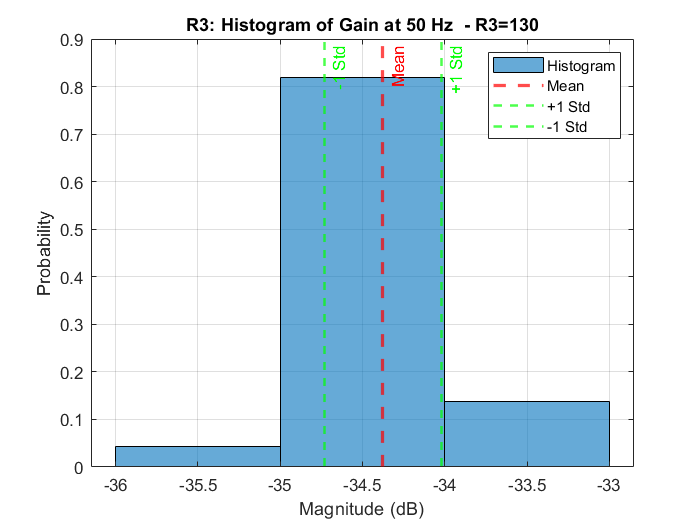
\includegraphics[width=\textwidth]{figures/r3=130/r3.png}
					\caption{$R_3$}
				\end{subfigure} \\
				
				\begin{subfigure}[h]{0.4\textwidth}
					\centering
					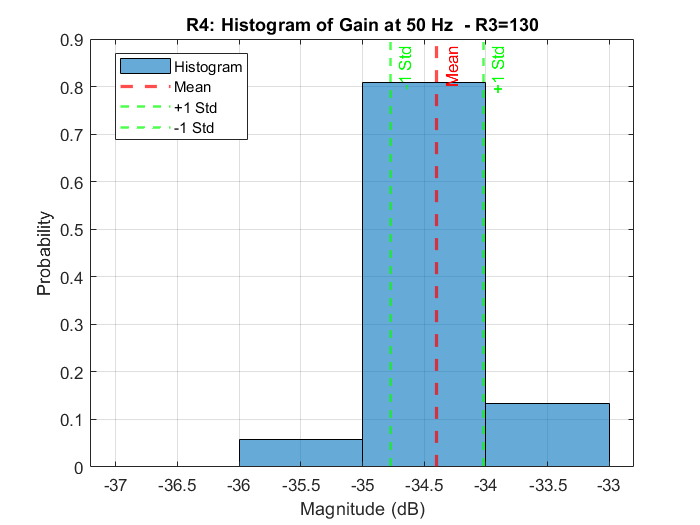
\includegraphics[width=\textwidth]{figures/r3=130/r4.png}
					\caption{$R_4$}
				\end{subfigure}
				\hfill
				\begin{subfigure}[h]{0.4\textwidth}
					\centering
					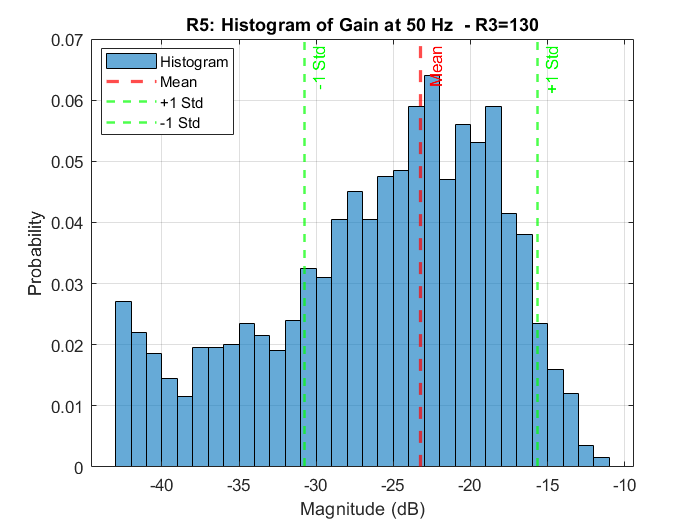
\includegraphics[width=\textwidth]{figures/r3=130/r5.png}
					\caption{$R_5$}
				\end{subfigure}
				\hfill
				\begin{subfigure}[h]{0.4\textwidth}
					\centering
					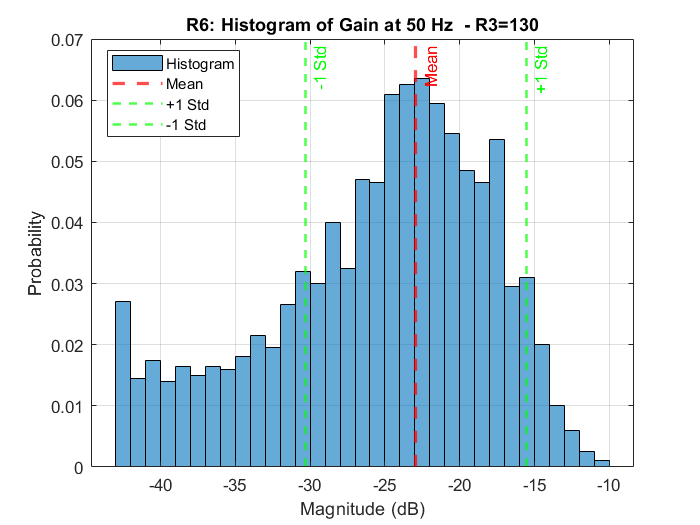
\includegraphics[width=\textwidth]{figures/r3=130/r6.png}
					\caption{$R_6$}
				\end{subfigure}
			\end{tabular}
		}
		\caption{Gain Histograms for Resistors with 5\% Tolerance}
	\end{figure}
	
	
	
	
	\pagebreak
	
	
	
	\subsubsection{$R_3 = 150\Omega$}
	
	\begin{figure}[!h]
		\centering
		\resizebox{0.75\textwidth}{!}{
			\begin{tabular}{c}
				\begin{subfigure}[h]{0.4\textwidth}
					\centering
					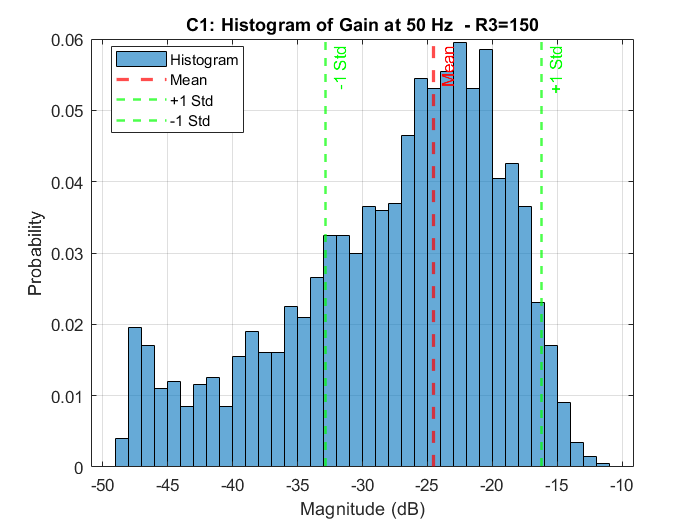
\includegraphics[width=\textwidth]{figures/r3=150/c1.png}
					\caption{$C_1$}
				\end{subfigure}
				\hfill
				\begin{subfigure}[h]{0.4\textwidth}
					\centering
					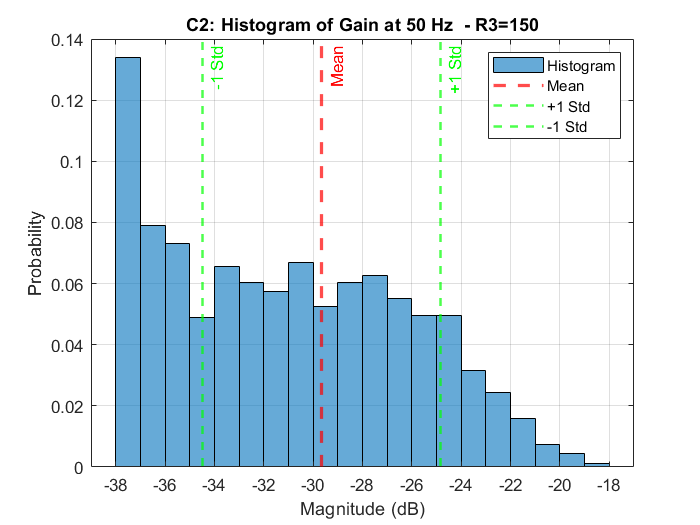
\includegraphics[width=\textwidth]{figures/r3=150/c2.png}
					\caption{$C_2$}
				\end{subfigure} \\
				
				\begin{subfigure}[h]{0.4\textwidth}
					\centering
					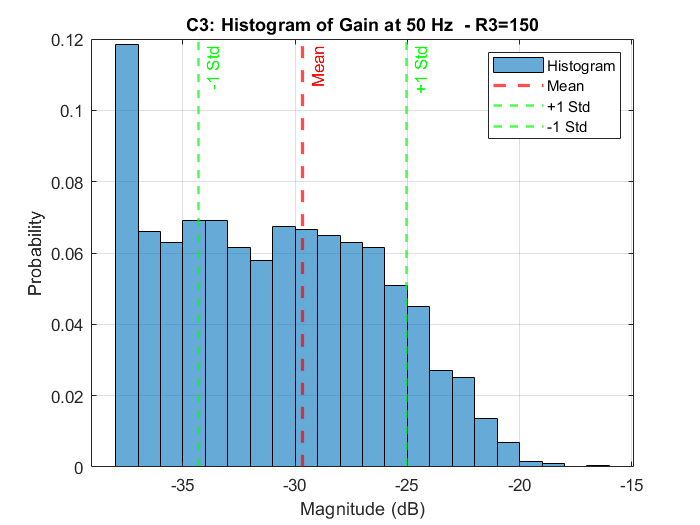
\includegraphics[width=\textwidth]{figures/r3=150/c3.png}
					\caption{$C_3$}
				\end{subfigure}
				\hfill
				\begin{subfigure}[h]{0.4\textwidth}
					\centering
					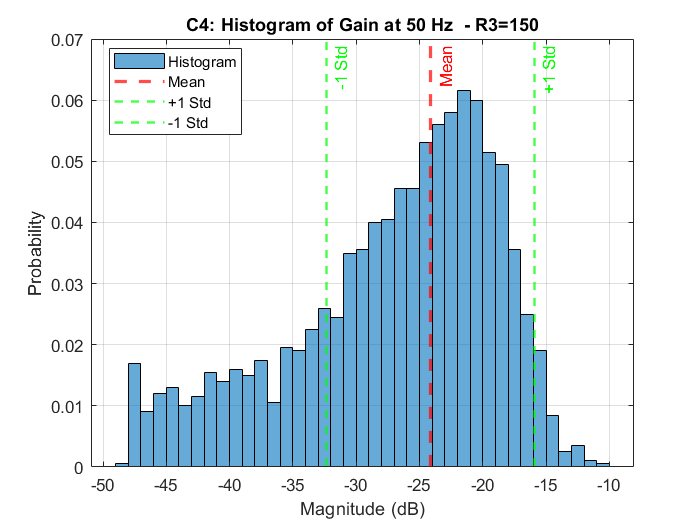
\includegraphics[width=\textwidth]{figures/r3=150/c4.png}
					\caption{$C_4$}
				\end{subfigure}
			\end{tabular}
		}
		\caption{Gain Histograms for Capacitors with 5\% Tolerance}
		\label{fig:R3_150_capacitors_5_percent}
	\end{figure}
	
	
	
	
	\begin{figure}[!h]
		\centering
		\resizebox{0.75\textwidth}{!}{
			\begin{tabular}{c}
				\begin{subfigure}[h]{0.4\textwidth}
					\centering
					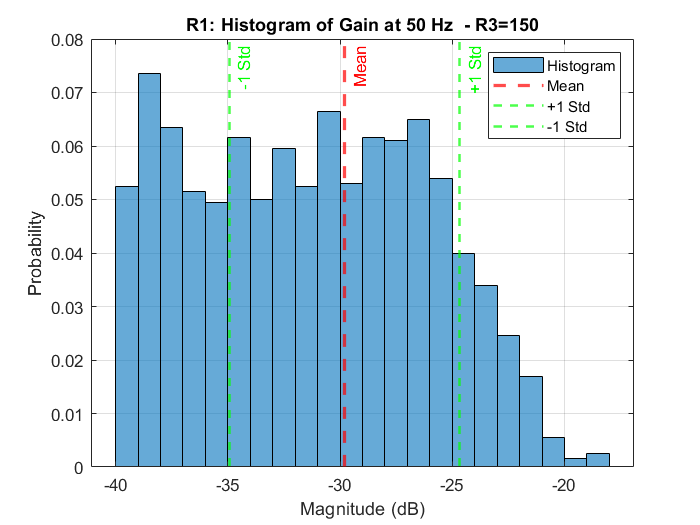
\includegraphics[width=\textwidth]{figures/r3=150/r1.png}
					\caption{$R_1$}
				\end{subfigure}
				\hfill
				\begin{subfigure}[h]{0.4\textwidth}
					\centering
					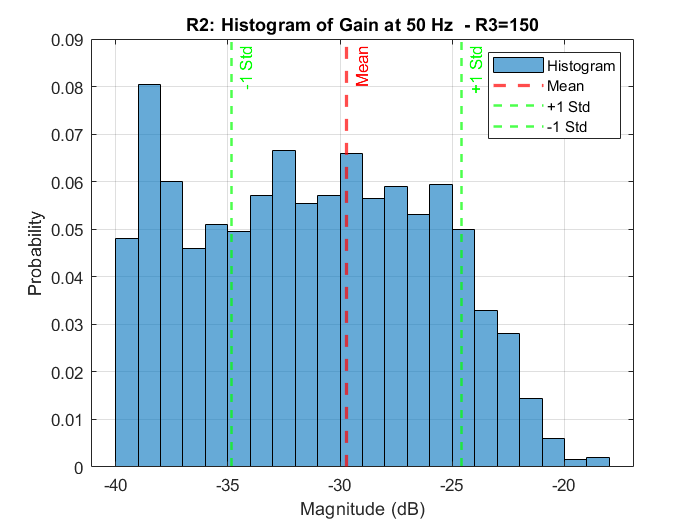
\includegraphics[width=\textwidth]{figures/r3=150/r2.png}
					\caption{$R_2$}
				\end{subfigure}
				\hfill
				\begin{subfigure}[h]{0.4\textwidth}
					\centering
					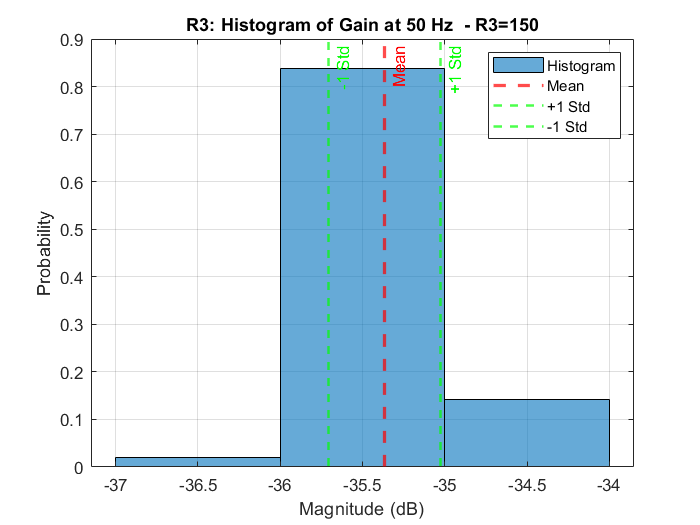
\includegraphics[width=\textwidth]{figures/r3=150/r3.png}
					\caption{$R_3$}
				\end{subfigure} \\
				
				\begin{subfigure}[h]{0.4\textwidth}
					\centering
					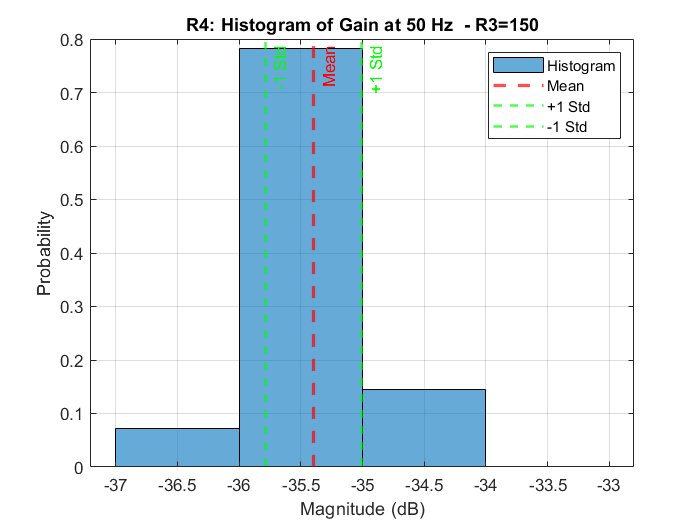
\includegraphics[width=\textwidth]{figures/r3=150/r4.png}
					\caption{$R_4$}
				\end{subfigure}
				\hfill
				\begin{subfigure}[h]{0.4\textwidth}
					\centering
					\includegraphics[width=\textwidth]{figures/r3=150/r5.png}
					\caption{$R_5$}
				\end{subfigure}
				\hfill
				\begin{subfigure}[h]{0.4\textwidth}
					\centering
					\includegraphics[width=\textwidth]{figures/r3=150/r6.png}
					\caption{$R_6$}
				\end{subfigure}
			\end{tabular}
		}
		\caption{Gain Histograms for Resistors with 5\% Tolerance}
		\label{fig:R3_150_resistors_5_percent}
	\end{figure}
	
	
	\pagebreak
	
	
	\subsubsection{Comparison}
	In this section, we determine \( P(\text{gain at 50\,Hz} < -20\,\text{dB}) \) by calculating the area under the histogram plot.
	
	\begin{table}[h!]
		\centering
		\begin{tabular}{c|c|c|c|c|c|c|c|c|c|c|}
			\cline{2-11}
			& $R_1$ & $R_2$ & $R_3$ & $R_4$ & $R_5$ & $R_6$ & $C_1$ & $C_2$ & $C_3$ & $C_4$ \\ \hline
			\multicolumn{1}{|c|}{$R_3=130$} & 99    & 99    & 100   & 100   & 75.2  & 75.2    & 72.6  & 98.3    & 98.5    & 74    \\ \hline
			\multicolumn{1}{|c|}{$R_3=150$} & 99.5  & 99.5  & 100   & 100   & 80    & 79    & 83.5  & 99.5    & 99.7  & 80.4  \\ \hline
		\end{tabular}
		\caption{P(gain at 50~Hz $<$ -20~dB)}
		\label{tab:pg50}
	\end{table}
	
	We can clearly see that \(150\,\Omega\) has improved the system in terms of probability compared to \(130\,\Omega\). Additionally, as we discussed earlier, variations in \( \{R_5, R_6, C_1, C_4\} \) have a more significant impact on the circuit's performance.
	
	
	\subsection{Finding the Maximum Tolerance for Each Element (\( R_3 = 150 \))}
	When looking at Table \textcolor{Cyan}{\ref{tab:pg50}}, we realize that not all of the elements met the requirement \textcolor{Cyan}{\ref{eq:constraints}}. For the elements that did meet these criteria, we can conclude that a 5\% tolerance is sufficient. However, for those that did not, we now perform a new simulation with a 2\% tolerance to determine if it will suffice, as 2\% is the next common tolerance after 5\%.
	
	It is worth mentioning that the results with a 5\% tolerance were not significantly below the threshold, with accuracy values around 0.85.
	
	
	\begin{figure}[!h]
		\centering
		\resizebox{0.75\textwidth}{!}{
			\begin{tabular}{c}
				\begin{subfigure}[h]{0.4\textwidth}
					\centering
					\includegraphics[width=\textwidth]{figures/2_percent/c1.png}
					\caption{$C_1$}
				\end{subfigure}
				\hfill
				\begin{subfigure}[h]{0.4\textwidth}
					\centering
					\includegraphics[width=\textwidth]{figures/2_percent/c4.png}
					\caption{$C_4$}
				\end{subfigure} \\
				
				\begin{subfigure}[h]{0.4\textwidth}
					\centering
					\includegraphics[width=\textwidth]{figures/2_percent/r5.png}
					\caption{$R_5$}
				\end{subfigure}
				\hfill
				\begin{subfigure}[h]{0.4\textwidth}
					\centering
					\includegraphics[width=\textwidth]{figures/2_percent/r6.png}
					\caption{$R_6$}
				\end{subfigure}
			\end{tabular}
		}
		\caption{2\% Tolerance for Sensitive Elements}
	\end{figure}
	
	 Looking at the graphs, it is clear that \( P(\text{gain at 50\,Hz} < -20\,\text{dB})\) exceeds 99\%. This indicates that a 2\% tolerance is sufficient for the sensitive elements.

	
	\pagebreak


	Now, we plot the histogram of the gain at 50~Hz using the newly determined tolerances.
	
	\begin{figure}[h!]
		\centering
		\includegraphics[scale=0.6]{figures/new_tolerances/bode.png}
		\caption{Magnitude of the Transfer Function with New Tolerances}
	\end{figure}
	
	\begin{figure}[h!]
		\centering
		\includegraphics[scale=0.5]{figures/new_tolerances/histogram.png}
		\caption{Gain Histogram Around 50~Hz with New Tolerances}
	\end{figure}

	
	
	When comparing with Figure\,\textcolor{Cyan}{\ref{fig:2_percent_tolerance_all}} (all with 2\% tolerance), we can see that our circuit has improved in terms of probability. The key observation is that by slightly increasing the bandwidth, we can increase the tolerance and achieve better results. In this case, 6 out of 10 elements have a 5\% tolerance, while only 4 have a 2\% tolerance.
	
	\pagebreak
	
	
	\subsection{Enhancing Circuit Robustness}
	We found that \(\{R_5, R_6, C_1, C_4\}\) are more sensitive to changes. In the previous section, we addressed this by lowering their tolerance. In this section, we explore another approach. As explained in Section~\textcolor{Cyan}{\ref{robust}}, we replace each resistor with two series-connected resistors of half the original value and each capacitor with two parallel-connected capacitors of half the original value with the same tolerance.
	
	
	\begin{figure}[!h]
		\centering
		\resizebox{0.75\textwidth}{!}{
			\begin{tabular}{c}
				\begin{subfigure}[h]{0.4\textwidth}
					\centering
					\includegraphics[width=\textwidth]{figures/robust/c1.png}
					\caption{$C_1$}
				\end{subfigure}
				\hfill
				\begin{subfigure}[h]{0.4\textwidth}
					\centering
					\includegraphics[width=\textwidth]{figures/robust/c4.png}
					\caption{$C_4$}
				\end{subfigure} \\
				
				\begin{subfigure}[h]{0.4\textwidth}
					\centering
					\includegraphics[width=\textwidth]{figures/robust/r5.png}
					\caption{$R_5$}
				\end{subfigure}
				\hfill
				\begin{subfigure}[h]{0.4\textwidth}
					\centering
					\includegraphics[width=\textwidth]{figures/robust/r6.png}
					\caption{$R_6$}
				\end{subfigure}
			\end{tabular}
		}
		\caption{Robust Circuit Approach}
	\end{figure}
	
	Comparing our results with Figure~\ref{fig:R3_150_capacitors_5_percent} and Figure~\ref{fig:R3_150_resistors_5_percent}, we observe that although all elements are assumed to have a 5\% tolerance in both cases, using the robust circuit method has significantly improved the results.
	
	\pagebreak
	
	
	\subsection{Question}
	Can you achieve a 20~dB attenuation with a probability of more than 90\% for all components with a 2\% tolerance and a bandwidth of 15~Hz? (If the answer is no, explain the reason for the limitation.)\\ \\
	First, we need to determine the value of \( R_3 \) for which the \(-3\,\text{dB}\) bandwidth equals 15~Hz. Through experimentation, we find that \( R_3 = 82\,\Omega \) is the closest value from the E24 series.
	
	\begin{figure}[!h]
		\centering
		\resizebox{0.8\textwidth}{!}{
		\begin{overpic}[width=1\textwidth]{figures/r3_82.png}
			\put(62,2){\includegraphics[width=0.35\textwidth]{figures/r3_82_caption.png}}
		\end{overpic}
		}
		\caption{Magnitude of Transfer Function, $R_3 = 82 \Omega$}
	\end{figure}
	
	To maximize our chances, we use the same method as in the previous section, replacing all elements with two series or parallel-connected components, each with half the original value, while maintaining a 2\% tolerance.
	
	\begin{figure}[!h]
		\centering
		\resizebox{1\textwidth}{!}{
			\begin{tabular}{c}
				\begin{subfigure}[h]{0.5\textwidth}
					\centering
					\includegraphics[width=\textwidth]{figures/question/histogram.png}
				\end{subfigure}
				\hfill
				\begin{subfigure}[h]{0.5\textwidth}
					\centering
					\includegraphics[width=\textwidth]{figures/question/bode.png}
				\end{subfigure}
			\end{tabular}
		}
		\caption{2\% Tolerance for All Elements}
	\end{figure}
	
	By examining the histogram plot, we observe that the probability of achieving more than 20~dB attenuation is approximately 58\%. Therefore, the answer is no, as it does not meet the required probability of over 90\%.
	
	\pagebreak
	
	\newpage
	
	\section{PCB Implementation}
	\subsection{Design}
	The images presented below show the PCB design of the notch filter circuit. The design was implemented using Altium Designer to create a compact and functional layout suitable for real-world implementation.
	
	\vspace{1cm}
	
	\begin{figure}[!h]
		\centering
			\begin{tabular}{c}
				\begin{subfigure}[h]{0.5\textwidth}
					\centering
					\includegraphics[width=\textwidth]{figures/altium/top_side_2d}
					\caption{Top-Side View, 2D Layout}
				\end{subfigure}
				\hfill
				\begin{subfigure}[h]{0.5\textwidth}
					\centering
					\includegraphics[width=\textwidth]{figures/altium/top_side_3d}
					\caption{Top-Side View}
				\end{subfigure} \\
				
				\begin{subfigure}[h]{0.5\textwidth}
					\centering
					\includegraphics[width=\textwidth]{figures/altium/isometric_view}
					\caption{Isometric View}
				\end{subfigure}
				\hfill
				\begin{subfigure}[h]{0.5\textwidth}
					\centering
					\includegraphics[width=\textwidth]{figures/altium/bottom_side}
					\caption{Bottom Side}
				\end{subfigure}
			\end{tabular}
	\end{figure}
	
	
	\pagebreak
	
	\subsection{Implementation}	 \label{sec:implementation}
	The resistors used in this project were purchased with a 5\% tolerance, and the capacitors were polyester capacitors, with a 10\% tolerance. Additionally, we used the NE5532 IC for the operational amplifier. Based on the available component values, the following resistor values were chosen for optimal performance:
	\\
	\begin{table}[ht]
		\centering
		\begin{tabular}{|c|c|c|c|}
			\hline
			\textbf{Resistor} & \textbf{Ideal Value (k\(\Omega\))} & \textbf{Value (k\(\Omega\))} & \textbf{Deviation from Ideal Value} \\ \hline
			$R_1$ & 680 & 677 & 0.44\% \\ \hline
			$R_2$ & 680 & 683 & 0.44\% \\ \hline
			$R_1$ $\parallel$ $R2$ & 340 & 339.993 & no significant difference \\ \hline
			$R_3$ & 0.150 & 0.1497 & 0.2\% \\ \hline
			$R_4$ & 1 & 0.989 & 1.1\% \\ \hline
			$R_5$ & 680 & 218.1 + 468 = 686.1 & 0.897\% \\ \hline
			$R_6$ & 680 & 217 + 464 = 681 & 0.147\% \\ \hline
		\end{tabular}
		\caption{Resistor Values and Deviations from Ideal Values}
	\end{table}
	
	\begin{table}[ht]
		\centering
		\begin{tabular}{|c|c|c|c|}
			\hline
			\textbf{Capacitor} & \textbf{Ideal Value (nF)} & \textbf{Value (nF)} & \textbf{Deviation from Ideal Value} \\ \hline
			$C1$ & 4.7 & 4.68 & \(0.43\%\) \\ \hline
			$C2$ & 4.7 & 4.74 & \(0.85\%\) \\ \hline
			$C3$ & 4.7 & 4.68 & \(0.43\%\) \\ \hline
			$C4$ & 4.7 & 4.71 & \(0.21\%\) \\ \hline
			$C_2 || C_3$ & 9.4 & 9.42 & \(0.21\%\) \\ \hline
		\end{tabular}
		\caption{Capacitor Values and Deviations from Ideal Values}
	\end{table}

	
	\begin{figure}[!ht]
		\centering
		\begin{subfigure}{0.45\textwidth}
			\centering
			\includegraphics[height=0.8\linewidth]{figures/results/implemented_circuit_image}
			\caption{Implemented Circuit}
		\end{subfigure}
		\hfill
		\begin{subfigure}{0.45\textwidth}
			\centering
			\includegraphics[height=0.8\linewidth]{figures/results/unassembled}
			\caption{Unassembled PCB Design}
		\end{subfigure}
	\end{figure}
	
	
	\pagebreak
	
	\subsection{Experimental Results}
	In this section, we analyze the performance of the implemented circuit by measuring its -3~dB cutoff frequencies and the amplitude of the output across a range of input frequencies. The input signal used for testing was:
	
	\[
	V_{\text{in}} = 1 + \sin(\omega t), \quad \omega = 2\pi f
	\]
	
	where \( f \) represents the frequency of the input signal.
	
	The \textbf{-3~dB cutoff frequency} is defined as the frequency at which the power of the output signal drops to half of its maximum value. This corresponds to a -3~dB reduction in amplitude, where the amplitude is measured in volts. Specifically, at the -3~dB point, the output voltage amplitude is approximately 0.707 times the maximum amplitude.
	
	In the following figures, the blue signal represents the input, while the yellow signal shows the output from our circuit. These images illustrate the circuit's performance at various frequencies.
	\\
	\begin{figure}[!h]
		\centering
		\begin{subfigure}[t]{0.45\textwidth}
			\centering
			\includegraphics[height=0.75\linewidth]{figures/results/38hz_double}
			\caption{DC-Coupled Output}
		\end{subfigure}
		\hfill
		\begin{subfigure}[t]{0.45\textwidth}
			\centering
			\includegraphics[height=0.75\linewidth]{figures/results/38hz_output_ac}
			\caption{AC-Coupled Output}
		\end{subfigure}
		\caption{Low-Frequency Cutoff, Approximately 38\,\text{Hz}}
	\end{figure}
	
	\begin{figure}[!h]
		\centering
		\begin{subfigure}{0.45\textwidth}
			\centering
			\includegraphics[height=0.75\linewidth]{figures/results/50hz_output_dc}
			\caption{DC-Coupled Output}
		\end{subfigure}
		\hfill
		\begin{subfigure}{0.45\textwidth}
			\centering
			\includegraphics[height=0.75\linewidth]{figures/results/50hz_output_ac}
			\caption{AC-Coupled Output}
		\end{subfigure}
		\caption{Notch Filter Frequency, Approximately 50\,\text{Hz}}
	\end{figure}
	
	\begin{figure}[!h]
		\centering
		\begin{subfigure}{0.45\textwidth}
			\centering
			\includegraphics[width=\linewidth]{figures/results/64hz_double}
			\caption{DC-Coupled Output}
		\end{subfigure}
		\hfill
		\begin{subfigure}{0.45\textwidth}
			\centering
			\includegraphics[width=\linewidth]{figures/results/64hz_output_dc}
			\caption{DC-Coupled Output}
		\end{subfigure}
		\caption{High-Frequency Cutoff, Approximately 64\,\text{Hz}}
	\end{figure}
	
	\pagebreak
	
	From the images presented above, we can have the following key observations:
	
	\begin{itemize}
		\item The low-frequency cutoff is observed at approximately 38~Hz.
		\item The notch filter is most effective around 50~Hz, where it attenuates the input signal by approximately -20.5~dB.
		\item The high-frequency cutoff is observed at approximately 63~Hz.
		\item -3~dB bandwidth is approximately 2~Hz.
	\end{itemize}
	
	Thus, we can conclude that the project requirements have been met.
	\begin{equation}
		\text{Requirements: } BW_{-3 \, dB} \le 25 \, \text{Hz}, \quad f_o = 50 \, \text{Hz}, \quad \text{Gain}(f = f_o) \le -20 \, \text{dB}
	\end{equation}
	
	
	\section{Appendix}
	\subsection{Measurement Equipment}
	\begin{itemize}
		\item \textbf{GDS-1062A Oscilloscope (GW Instek)}: To capture and record the input and output signals of the circuit.
		
		\item \textbf{GDM-396 Multimeter (GW Instek)}: To measure key circuit parameters such as voltage, current, and resistance.
		
		\item \textbf{SFG-1013 Function Generator (GW Instek)}: To generate the test input signal.
		
		\item \textbf{LCR-821 LCR Meter (GW Instek)}: To measure capacitor values accurately.
	\end{itemize}
	
	\bibliographystyle{ieeetr}
	\bibliography{references}
	
\end{document}
